\documentclass{standalone}

\usepackage{tikz}
\usetikzlibrary{angles,quotes}
\usepackage{amsmath,amssymb,amsfonts}

\usepackage{pgfplots}
\definecolor{darkgreen}{rgb}{0.0, 0.42, 0.24}
\definecolor{amethyst}{rgb}{0.6, 0.4, 0.8}

\pgfplotsset{compat=newest}
\pgfplotsset{every axis/.append style={
                     tick label style={font=\footnotesize},
                 }}


\begin{document}
    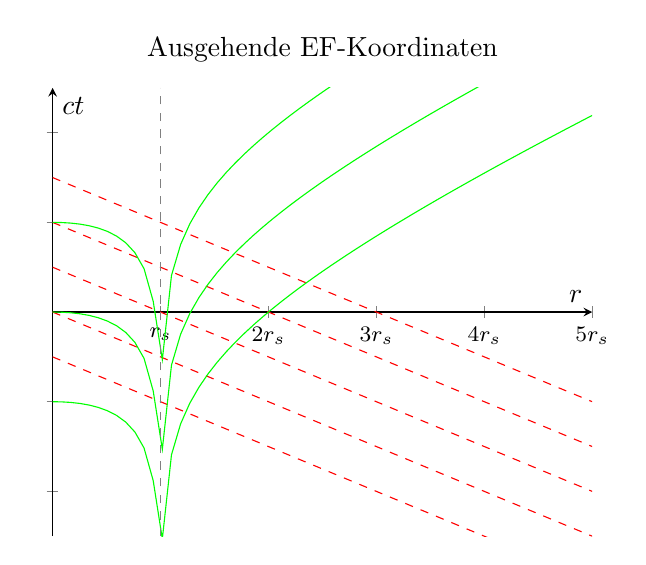
\begin{tikzpicture}
        \begin{axis}[title=$\text{Ausgehende EF-Koordinaten}$,xmin=0,xmax=5,ymin=-5,ymax=5,
        xtick={0,1,2,3,4,5},
        xticklabels={$0$,$r_{s}$,$2r_{s}$,$3r_{s}$,$4r_{s}$,$5r_{s}$},
        yticklabels=false,
        axis lines = middle,
        xlabel=$r$,
        ylabel=$ct$,
        domain=0:5]
            \addplot[color=red,dashed,samples=6]{-x+3};
            \addplot[color=red,dashed,samples=6]{-x+2};
            \addplot[color=red,dashed,samples=6]{-x+1};
            \addplot[color=red,dashed,samples=6]{-x};
            \addplot[color=red,dashed,samples=6]{-x-1};
            \addplot[color=green,samples=60]{2(x+ln(abs(x-1)))};
            \addplot[color=green,samples=60]{2(x+ln(abs(x-1)))+2};
            \addplot[color=green,samples=60]{2(x+ln(abs(x-1)))-2};
           \addplot[color=gray,dashed,samples=3] coordinates {(1,-5)(1,5)};
        \end{axis}
    \end{tikzpicture}
\end{document}